\documentclass[14pt, oneside]{article} % Default font size and left-justified equations
\usepackage[top=3cm,bottom=3cm,left=3.2cm,right=3.2cm,headsep=10pt]{geometry} % Page margins
\usepackage{xcolor} % Required for specifying colors by name
\definecolor{ocre}{RGB}{243,102,25} % Define the orange color used for highlighting throughout the book
\usepackage{avant} % Use the Avantgarde font for headings
\usepackage{mathptmx} % Use the Adobe Times Roman as the default text font together with math symbols from the Sym­bol, Chancery and 
\usepackage{microtype} % Slightly tweak font spacing for aesthetics
\usepackage[utf8]{inputenc} % Required for including letters with accents
\usepackage[T1]{fontenc} % Use 8-bit encoding that has 256 glyphs
\usepackage{titlesec} % Allows customization of titles
\usepackage{graphicx} % Required for including pictures
\usepackage{subcaption}
\captionsetup{justification=raggedright,singlelinecheck=false}
\graphicspath{{Pictures/}} % Specifies the directory where pictures are stored
\usepackage{tikz} % Required for drawing custom shapes
\usepackage[french]{babel} % English language/hyphenation
\usepackage{enumitem} % Customize lists
\setlist{nolistsep} % Reduce spacing between bullet points and numbered lists
\usepackage{booktabs} % Required for nicer horizontal rules in tables
\usepackage{eso-pic}
\usepackage{url}
\usepackage{parskip}
% Bibliography

%--------color de portada-----------------
\definecolor{titlepagecolor}{cmyk}{1,.60,0,.40}
\definecolor{namecolor}{cmyk}{0,0,0,0}
\definecolor{titlecolor}{RGB}{255,127,36}
\definecolor{liccolor}{RGB}{32,178,170}
%--------color de portada-----------------
\begin{document}
	
	%----------------------------------------------------------------------------------------
	%    TITLE PAGE
	%----------------------------------------------------------------------------------------
	
	\begingroup
	\begin{titlepage}
		\newgeometry{left=2.5cm,top=0cm,bottom=2.5cm, right=2.5cm}
		\AddToShipoutPicture*{\put(0,0){\includegraphics[scale=1]{RapportPortada.pdf}}} % Image background
		\noindent
		\vspace{5mm}
	\end{titlepage}
	\endgroup
	
	%----------------------------------------------------------------------------------------
	%    TABLE OF CONTENTS
	%----------------------------------------------------------------------------------------
	\cleardoublepage
	\pagestyle{empty} % No headers
	\tableofcontents % Print the table of contents itself
	\cleardoublepage % Forces the first chapter to start on an odd page so it's on the right
	
	
	%----------------------------------------------------------------------------------------
	%    CHAPTER 1
	%----------------------------------------------------------------------------------------
	\newpage
	
	\section{Introduction}
		\paragraph
		De nombreuses personnes meurent chaque année dans des accidents de la route. Et la raison de ces accidents c’est presque toujours le manque d’attention du côté du conducteur. Pendant ces dernières années il y a eu un grand intérêt dans le développement de systèmes de détection des piétons qui pourraient aider à reduire l'ampleur et l'impact de ces accidents. 
		La plupart des systèmes proposés utilisent une caméra comme capteur, car les caméras peuvent fournir la résolution nécessaire pour une classification et une mesure de position précises. Les caméras peuvent également être partagées avec d'autres sous-systèmes d'assistance à la sécurité dans la voiture, tels qu'un système d'assistance de maintien de voie, améliorant ainsi le rapport prix / avantages de la caméra.
		
		
	\section{Contexte}
		\paragraph
		Construire un modèle de réseaux de neurones capable de détecter et de suivre des piétons.
		Ce problème peut être abordé avec différentes approches 
		
	\section{Différentes approaches }
		\begin{itemize}
			\item CNN avec sliding windows \cite{SlidingWindows}
		\end{itemize}
		\begin{itemize}
			\item 	CNN avec OpenCv
		\end{itemize}
		\begin{itemize}
			\item 	Recurrent Convolutional Neural Network (R-CNN) \cite{RcnnFrcnnYolo}
		\end{itemize}
		\begin{itemize}
			\item 	Fast Recurrent Convolutional Neural Network (Fast R-CNN) \cite{RcnnFrcnnYolo}
		\end{itemize}
		\begin{itemize}
			\item 	Faster Recurrent Convolutional Neural Network (Faster R-CNN) \cite{RcnnFrcnnYolo}
		\end{itemize}
		\begin{itemize}
			\item 	You Only Look Once (YOLO) \cite{RcnnFrcnnYolo} \cite{yolov3}
		\end{itemize}
		
	\section{Approche utilisée}
		\paragraph
			Dans ce travail j’ai utilisé un CNN avec OpenCv. Le CNN je l’ai utilisé pour faire un « image classifier » et OpenCv pour le traitement des images. Totu cela a été fait en Python et Keras pour le CNN
		\subsection{Qu’est-ce qu’un CNN est? }
		\paragraph
			En deep learning, un réseau de neurones convolutifs ou réseau de neurones à convolution (en anglais CNN ou ConvNet pour Convolutional Neural Networks) est un type de réseau de neurones artificiels, dans lequel le motif de connexion entre les neurones est inspiré par le cortex visuel des animaux. Les neurones de cette région du cerveau sont arrangés de sorte qu'ils correspondent à des régions qui se chevauchent lors du pavage du champ visuel. Leur fonctionnement est inspiré par les processus biologiques, ils consistent en un empilage multicouche de perceptrons \footnote{Le perceptron est un algorithme d'apprentissage supervisé de classifieurs binaires (c'est-à-dire séparant deux classes)} , dont le but est de prétraiter de petites quantités d'informations. Les réseaux neuronaux convolutifs ont de larges applications dans la reconnaissance d'image et vidéo, les systèmes de recommandation et le traitement du langage naturel. 
			\begin{figure}
				\centering
				\includegraphics[width=0.7\textwidth]{cnnExample}
				\caption{Example d'un CNN}
			\end{figure}	
		\subsection{Qu’est-ce que OpenCv est ?}
			\paragraph
				OpenCV (pour Open Computer Vision)  \cite{OpenCv} est une bibliothèque graphique libre, initialement développée par Intel, spécialisée dans le traitement d'images en temps réel.
		\subsection{Qu’est-ce que Keras est ?}
			\paragraph
				Keras \cite{Keras} est une bibliothèque de réseau de neurones open source écrite en Python. Il est capable de fonctionner sur TensorFlow \cite{tensorflow}, Microsoft Cognitive Toolkit ou Theano. Elle a été conçue pour permettre une expérimentation rapide avec des réseaux de neurones profonds.
	\section{Mise en oeuvre }
		\paragraph
			Pour ce travail j’ai utilisé différents mod\`{e}les de CNN entrainés avec différentes images de tailles différentes. Une fois le  mod\`{e}le entrainé, j’ai utilisé OpenCv pour lire une video (frame par frame), soustraire le fond du frame actuel et retrouver les contours des objects sur l’image. Une fois cela fait je modifie la taille de l’image pour pouvoir utiliser mon resseau de neurones et identifier si dans l’image il y a un piéton ou non. Dans le cas positif je dessine un bounding box autour du piéton identifié. 
	\section{Différents  mod\`{e}les}
		\paragraph
			J’ai entrainé 3 resseau de neurones différents avec des différentes images de différentes tailles. Chaque groupe d’images a été divisé en TrainingData et ValidationData (ValidationData = 10 \% ou 20\% du TrainingData).
		\subsection{CNN 150x150 avec Kitti}
			\paragraph
				Le premier CNN je l’ai entrainé avec des images du dataset KITTI \cite{Geiger2012CVPR} . Ce dataset est compos\'{e} de 7481 images de 1242x375 pixels qu’ont été transformées de RGB à noir et blanc. Dans le ValidationData j’ai mis 748 images et dans le TrainingData j’ai mis 6733. Finalement j’ai separ\'{e} chaque set de donn\'{e}es en Pedestrian et NonPedestrian.
				Puis avant d’entrainer le resseau j’ai modifié la taille des images de 1242x375 pixels à 150x150 pixels, de cette façon l’entrainement se fait beaucoup plus rapide. 
							
			\subsubsection{Dataset}
				
				\begin{figure}[h!]
					\raggedright
					\begin{subfigure}[b]{0.4\textwidth}
					\includegraphics[width=\textwidth]{kitti/kittiImgRGBPed}
					\caption{Image avant modification des couleurs}
				\end{subfigure}	
			~
				\begin{subfigure}[b]{0.4\textwidth}	
					\includegraphics[width=\textwidth]{kitti/kittiImgGrayPed}
					\caption{Image apr\`{e}s modification des couleurs}
				\end{subfigure}	
			
				\begin{subfigure}[b]{0.4\textwidth}
					\includegraphics[width=\textwidth]{kitti/kittiImgGrayPed}
					\caption{Image avec des pi\'{e}tons}
				\end{subfigure}
			~
				\begin{subfigure}[b]{0.4\textwidth}
					\includegraphics[width=\textwidth]{kitti/kittiImgGrayNoPed}
					\caption{Image sans pi\'{e}tons}
				\end{subfigure}	
				\caption{Images du dataset Kitti}
			\end{figure}
		\newpage
			\subsubsection{Structure du resseau}
			\begin{figure}[h]
				\raggedright
				\includegraphics[width=0.7\textwidth]{kitti/structure}
				\caption{Structure du resseau}
			\end{figure}
		
		\subsection{CNN 18x36 avec Daimler}
			\paragraph
				Pour le 2eme CNN j’ai utilisé des images du dataset Daimler \cite{DaimlerDataset} . Ce dataset est compos\'{e} de 7840 images dans le TrainingData et 1960 images dans le ValidationData. Dans ce cas, les images on \'{e}t\'{e} aussi separ\'{e}es entre Pedestrian et NonPedestrian dans chacun des set des donn\'{e}es. Les images de ce dataset sont des images de 18X36 pixels en noir et blanc (Figure \ref{daimlerImagesSmall}) . Les images n’ont pas été modiffiées et avec ce model j’ai eu une précision du 80\% environ (Figure \ref{pertesPrecisionDaimlerSmall}) 
				
			\subsubsection{Dataset}
				\newpage
				\begin{figure}[h!]
					\raggedright
					\begin{subfigure}[b]{0.4\textwidth}
						\includegraphics[width=0.7\textwidth]{kitti/daimlerSmallNoPed}
						\caption{Image sans pi\'{e}tons}
					\end{subfigure}	
					~
					\begin{subfigure}[b]{0.4\textwidth}	
						\includegraphics[width=0.7\textwidth]{kitti/daimlerSmallPed}
						\caption{Image avec des pi\'{e}tons}
					\end{subfigure}	
					\caption{Images du dataset Daimler 18x36}
					\label{daimlerImagesSmall}
				\end{figure}
				
			\subsubsection{Pertes et précision}
				\begin{figure}[h!]
					\raggedright
					\begin{subfigure}[b]{0.5\textwidth}
						\includegraphics[width=\textwidth]{newplot(2)}
						\caption{Perte}
					\end{subfigure}	
					~
					\begin{subfigure}[b]{0.5\textwidth}	
						\includegraphics[width=\textwidth]{newplot(3)}
						\caption{Precision}
					\end{subfigure}	
					\caption{Pertes et précision}
					\label{pertesPrecisionDaimlerSmall}
				\end{figure}
			\subsubsection{Structure du resseau}
				\begin{figure}[h!]
					\raggedright
					\includegraphics[width=0.7\textwidth]{ped-18x36/structure}
					\caption{Structure du resseau}
				\end{figure}
			\newpage
		\subsection{CNN 64x64 avec Daimler}
			\paragraph
				Pour le 3eme et dernier CNN j’ai utilisé les mêmes images que pour le 2eme CNN mais avec une taille de 64X64 pixels (Figure \ref{daimlerImgBigger}) . Avec ce mod\`{e}le j’ai eu une précision du 89\% environ (Figure \ref{PertesPrecisionBigger}) . 
				
			\subsubsection{Dataset}
			\newpage
				\begin{figure}[h!]
					\raggedright
					\begin{subfigure}[b]{0.4\textwidth}
						\includegraphics[width=\textwidth]{kitti/daimlerBiggerNoPed}
						\caption{Image sans pi\'{e}tons}
					\end{subfigure}	
					~
					\begin{subfigure}[b]{0.4\textwidth}	
						\includegraphics[width=\textwidth]{kitti/daimlerBiggerPed}
						\caption{Image avec des pi\'{e}tons}
					\end{subfigure}	
					\caption{Images du dataset Daimler 64x64 px}
					\label{daimlerImgBigger}
				\end{figure}
				
			\subsubsection{Pertes et précision}
				\begin{figure}[h!]
					\raggedright
					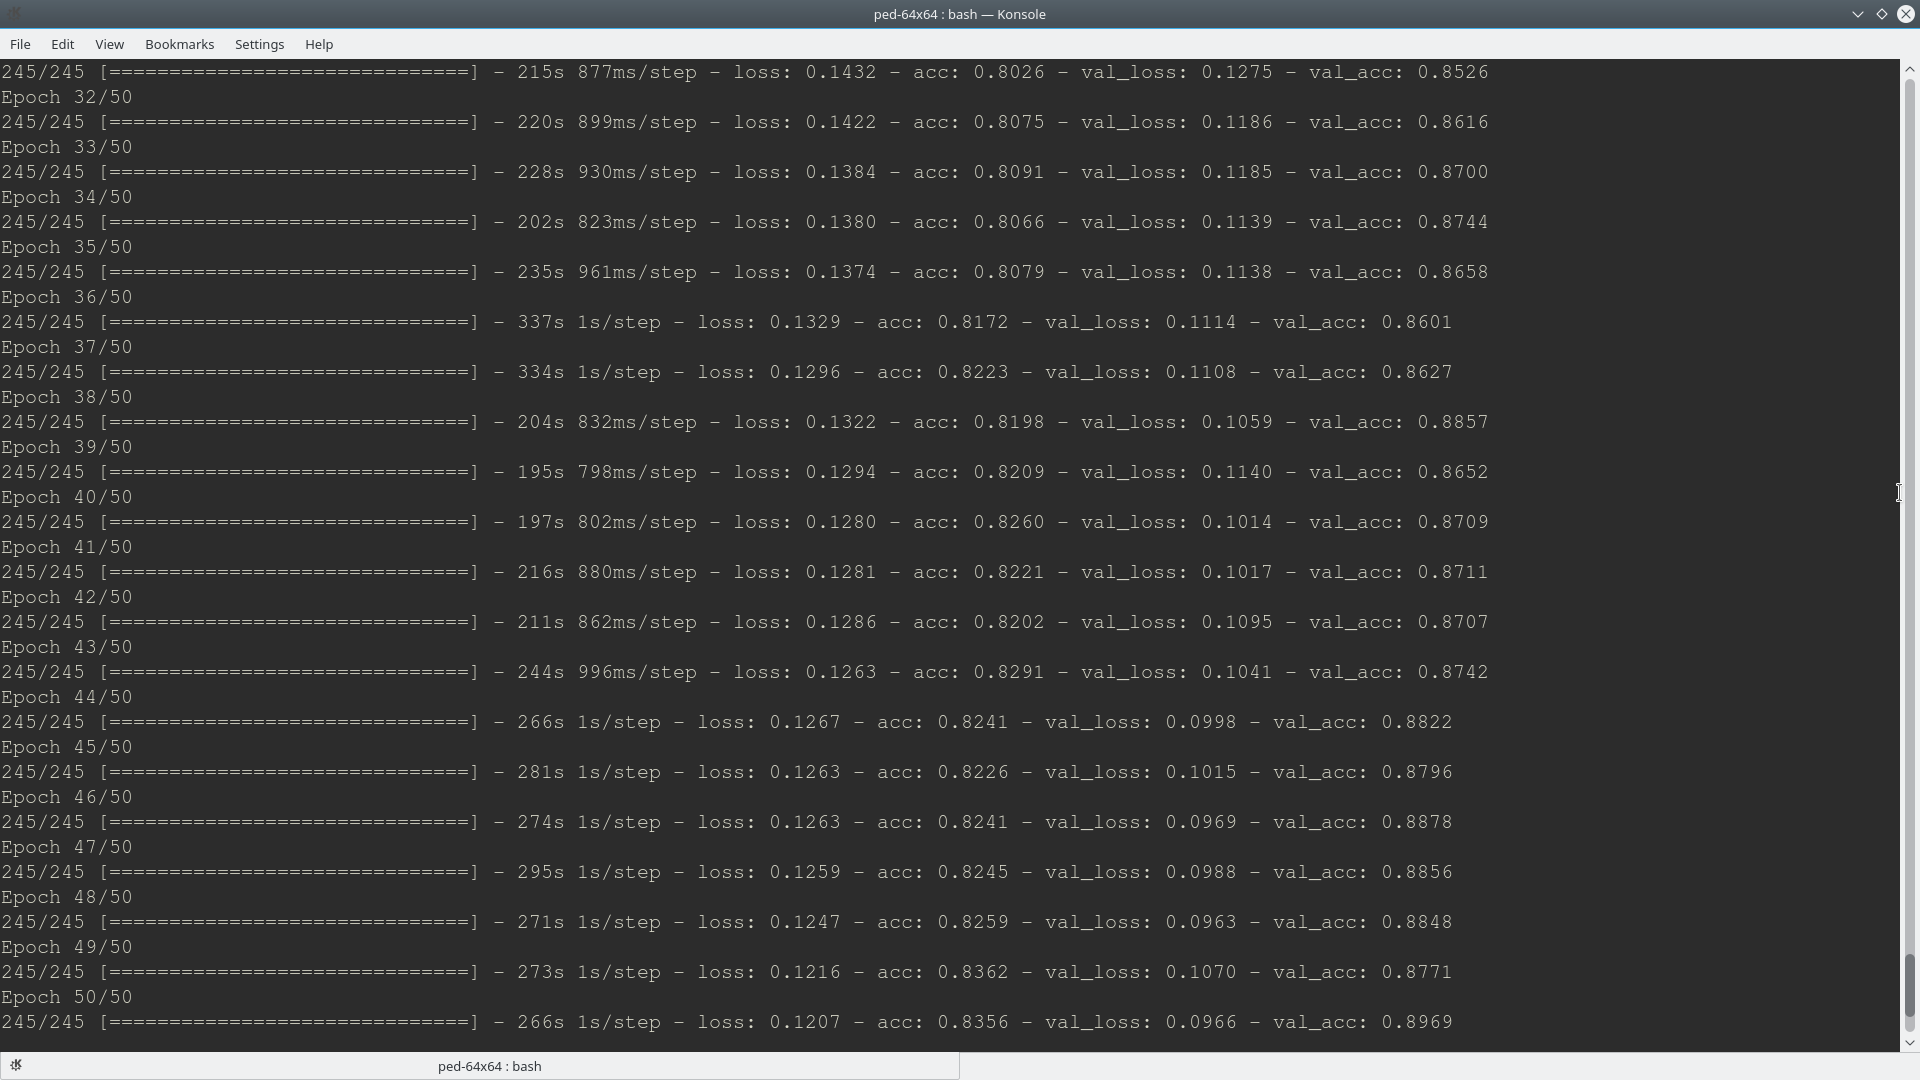
\includegraphics[width=\textwidth]{ped-64x64/consoleLogs}
					\caption{Pertes et précision}
					\label{PertesPrecisionBigger}
				\end{figure}
				\newpage
			\subsubsection{Structure du resseau}
				\begin{figure}[h!]
					\raggedright
					\includegraphics[width=0.8\textwidth]{ped-64x64/structure}
					\caption{Structure du resseau}
				\end{figure}		
				\newpage
		\subsection{Code pour construire les resseaux de neurones}
		
			\subsubsection{CNN 150x150}

					\includegraphics[width=0.9\textwidth]{code150x150}

			\subsubsection{CNN 18x36}
				\includegraphics[width=1.05\textwidth]{code18x36}

			
			\subsubsection{CNN 64x64}
				\includegraphics[width=1.05\textwidth]{code64x64}
		\subsection{Entrainement des CNN}
			\subsubsection{CNN 150x150}
				\includegraphics[width=0.9\textwidth]{trainkitti1}
				
				\includegraphics[width=0.9\textwidth]{trainkitti2}
			\subsubsection{CNN 18x36}
					\includegraphics[width=0.9\textwidth]{training18x362}
					
					\includegraphics[width=0.9\textwidth]{training18x361}
			\subsubsection{CNN 64x64}
					\includegraphics[width=0.9\textwidth]{training64x642}
					
					\includegraphics[width=0.9\textwidth]{training64x641}
					
	\section{Suivi des pi\'{e}tons}
		\paragraph
		Pour le suivi des pi\'{e}tons j’ai utilis\'{e} openCv et mon CNN. Tout d’abord j’ouvre une vid\'{e}o et j’enregistre chaque frame dans une variable.
		
			\includegraphics[width=0.9\textwidth]{suivi1}
			
		Apr\`{e}s je charge le mod\`{e}le \`{a}  utiliser et j’enl\`{e}ve le background du frame (Figure \ref{noBackground}) .
		
			\includegraphics[width=0.9\textwidth]{suivi2} 
	
		\begin{figure}[h!]
			\raggedright
			\includegraphics[width=0.9\textwidth]{suivi3}
			\caption{Image du frame sans background}
			\label{noBackground}
		\end{figure}
		
		Puis je fais un peu de traitement d’image sur le frame (expansion et débruitage) et je trouve les contours des objects pr\'{e}sents sur le frame (findContours).
		
			\includegraphics[width=0.9\textwidth]{suivi4} 
			
		 Finalement j’extrais les objects sur l’image et j’utilise mon resseau de neurones pour classifier s'il y a un pi\'{e}ton ou pas.
		 
		  	\includegraphics[width=0.9\textwidth]{suivi5}
		  
		  	\includegraphics[width=0.9\textwidth]{suivi6}
		  
		  S'il y a un pi\'{e}ton je dessine un bounding box autour de l’object et s'il n'y a pas de pi\'{e}ton je ne dessine pas de bounding box
		  
		  	\includegraphics[width=0.9\textwidth]{suivi7}
		  	
		  Apr\`{e}s je montre le frame avec ou sans le bounding box dessiné
		  
		  	\includegraphics[width=0.9\textwidth]{suivi8}
		  	\newpage
	\section{R\'{e}sultats}
		\paragraph
			Pour tester la fonctionalité des mod\`{e}les, j'ai utilisé la vid\'{e}o de « town center video » avec les 3 mod\`{e}les.
		\subsection{Capture de la vid\'{e}o originale}
		
			\includegraphics[width=0.9\textwidth]{resultat1}
			
		\subsection{Capture de la vid\'{e}o apr\`{e}s le 1er  mod\`{e}le}
			
				\includegraphics[width=0.9\textwidth]{resultat2}
			
		\subsection{Capture de la vid\'{e}o  apr\`{e}s le 2eme  mod\`{e}le}
		
				\includegraphics[width=0.9\textwidth]{resultat3}
		
		\subsection{Capture de la vid\'{e}o  apr\`{e}s le 3eme  mod\`{e}le}
		
				\includegraphics[width=0.9\textwidth]{resultat4}
	
		
	
	%----------------------------------------------------------------------------------------
	%    BIBLIOGRAPHY
	%----------------------------------------------------------------------------------------
	\newpage
	\nocite{*}
	\bibliographystyle{siam}
	\bibliography{referencias}


\end{document}
